\documentclass{article}

\usepackage[final]{nips_2016}

\usepackage[utf8]{inputenc} % allow utf-8 input
\usepackage[T1]{fontenc}    % use 8-bit T1 fonts
\usepackage{hyperref}       % hyperlinks
\usepackage{url}            % simple URL typesetting
\usepackage{booktabs}       % professional-quality tables
\usepackage{amsfonts}       % blackboard math symbols
\usepackage{nicefrac}       % compact symbols for 1/2, etc.
\usepackage{microtype}      % microtypography
\usepackage{amsmath}
\usepackage{color,graphicx}

\title{Deep Learning --- Assignment 4}

\author{Anirudhan J.~Rajagopalan \\
  Department of Computer Science\\
  New York University\\
  New York, NY.\\
  \texttt{ajr619@nyu.edu} \\
}

\begin{document}

\maketitle

\section{nnGraph}
\subsection{1. Warmup}
The code for nngraph\_warmup.lua can be found at \url{https://git.io/vwQco}

\subsubsection{2. Grucell diagram}
The gru cell was drawn using the following steps.
\begin{enumerate}
  \item Code the cell in torch similar to the code in main.lua
  \item Plot the code using graph.dot function passing the filename argument
  \item Open the svg file in browser and remove the unwanted nodes.
\end{enumerate}

The cell diagram generated is included in~\ref{fig:gru_cell}.

\begin{figure}[ht!]
  \centering
  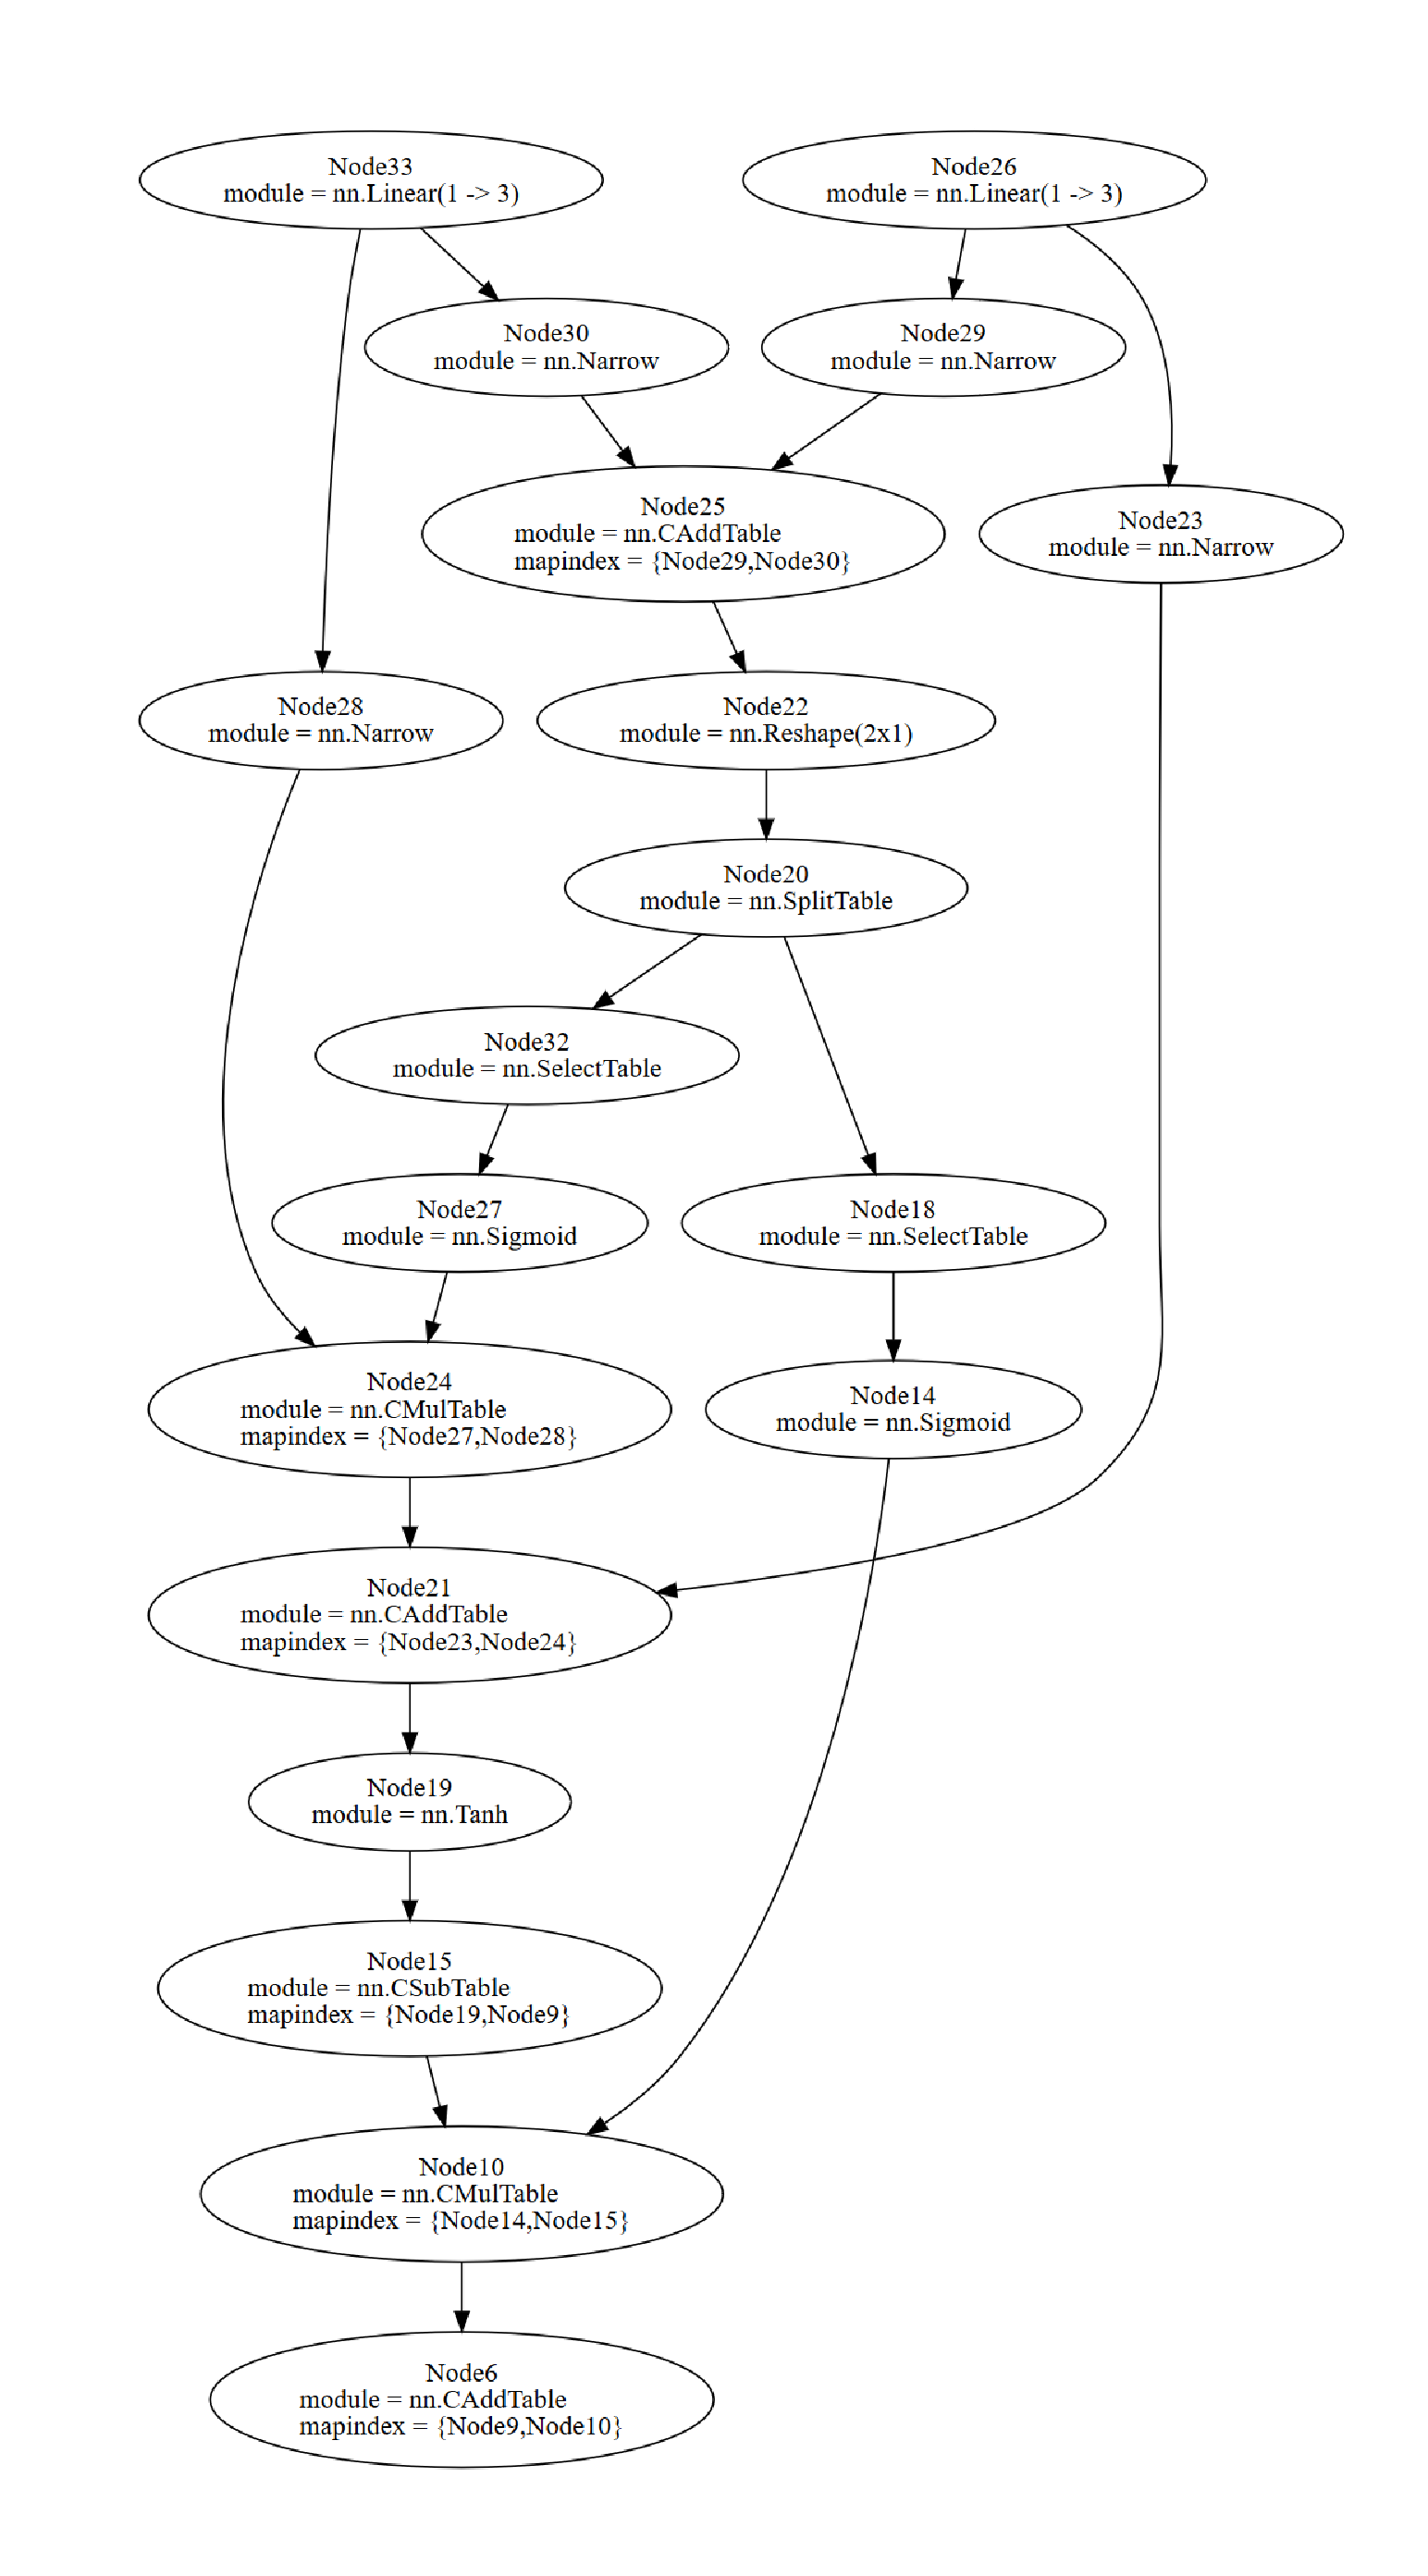
\includegraphics[height=1\textheight]{true}
  \caption{GRUCell given in slide 32 of talk by Armand Joulin\label{fig:gru_cell}}
\end{figure}

\section{Language Modeling}
\subsection{Generating sequences}
The query\_sentences.lua can be found at \url{https://git.io/vwQEc}.

The query\_sentences.lua does the following
\begin{enumerate}
  \item Loads the core network of the model.
  \item Builds the vocabulary map and the inverse vocabulary map.
  \item Fetches the number of words to generate and the initial seed words (minimum 2).
  \item Does a forward pass on the core\_network for each and every word to generate the index for next word.
  \item The index is generated by using a multinomial distribution over the probabilities generated by the logsoftmax layer (layer 44 in core\_network)
  \item Concatenates and returns the new sentence.
\end{enumerate}

Steps to run the model:  
\begin{enumerate}
  \item Change the params table in query\_sentences.lua accoding to the model that will be used.
  \item Change the model file path to point to the right path
  \item \textit{th query\_sentences.lua}
\end{enumerate}

\subsection{Improvements to the model}
\subsubsection{Experiments summary}
A number of experiments were preformed on the model.  A few of the major areas which we explored are
\begin{enumerate}
  \item Changing the size of rnn (200, 600).  The best performing model has rnn\_size of 600.
  \item Enabling/changing dropout.  The best performing model has a dropout of 
  \item Changing the sequence length.  The best performing model has a sequence length of 30.
  \item Changing the core network to work with GRU instead of lstm (Code can be found in \url{https://git.io/vwQXB})
  \item Chainging the number of layers.  Increasing the number of layers consistently decreased the performance of the model.
  \item Changing gradient clipping.  Changing the gradient clipping doesn't appear to affect the outputs much.
  \item Changing the vocabulary size.  This actually has no effect as the total number of words in the corpus is only 10,000.
\end{enumerate}

The best performing model has a test accuracy of \textbf{}.  The model characteristics are
\begin{description}
  \item[vocab\_size] 12000
  \item[core\_network] LSTM
  \item[Seq\_length] 30
  \item[rnn\_size] 600
  \item[dropout] 0.4
  \item[layers] 2
\end{description}


\subsubsection{Hardware \& Runtimes}
Almost all of the experiments were run in NYU HPC clusters with 20 core processors, 16GB RAM\@.

The default model ran ran fast with wps = 2K. There was considerable reduction in the speed of the model as the rnn\_size is increased. The best performing model has a wps of around 650.

\subsubsection{Model file}
The model file can be found at \url{http://cs.nyu.edu/~ajr619/lang\_model.net}

\subsubsection{Experiments}
LSTM
\begin{center}
\begin{tabular}{c c c c c c c} 
seq length & layers & rnn size & dropout  & vocab size & best Perplexity\\
 20 & 2 & 200 & 0 &  10000 & 119.756\\ 
 30 & 2 & 200 & 0 &  10000 & 114.548\\ 
 15 & 2 & 200 & 0 &  10000 & 195.712\\ 
  30 & 4 & 200 & 0 & 10000 & 120.359\\
  40 & 3 & 200 & 0 & 15000 & 137.629\\
 40 & 5 & 200 & 0.2 & 10000 & 135.020\\
 40 & 4 & 400 & 0.2 & 10000 & 107.970\\
 30 & 2 & 400 & 0.2 & 10000 & 93.449\\
 30 & 4 & 400 & 0.3 & 10000 & 102.013\\
  30 & 4 & 400 & 0.5 & 10000 & 113.420\\
  
  30 & 2 & 400 & 0.5 &  10000 & 96.340\\
  30 & 2 & 600 & 0.4 &  12000 & 87.741\\  
  30 & 2 & 500 & 0.3 &  10000 & 89.794\\  
   
\end{tabular}
\end{center}

GRU

\begin{center}
\begin{tabular}{c c c c c c c} 
seq length & layers & rnn size & dropout & vocab size & best Perplexity\\
 20 & 2 & 200 & 0 &  10000 & 182.217\\ 
 15 & 2 & 200 & 0 &  10000 & 195.712\\ 
 30 & 2 & 600 & 0.4 &  10000 & 97.056\\
 30 & 2 & 700 & 0.5 & 10000 & 101.021\\  
\end{tabular}
\end{center}

\begin{figure}[ht!]
  \centering
  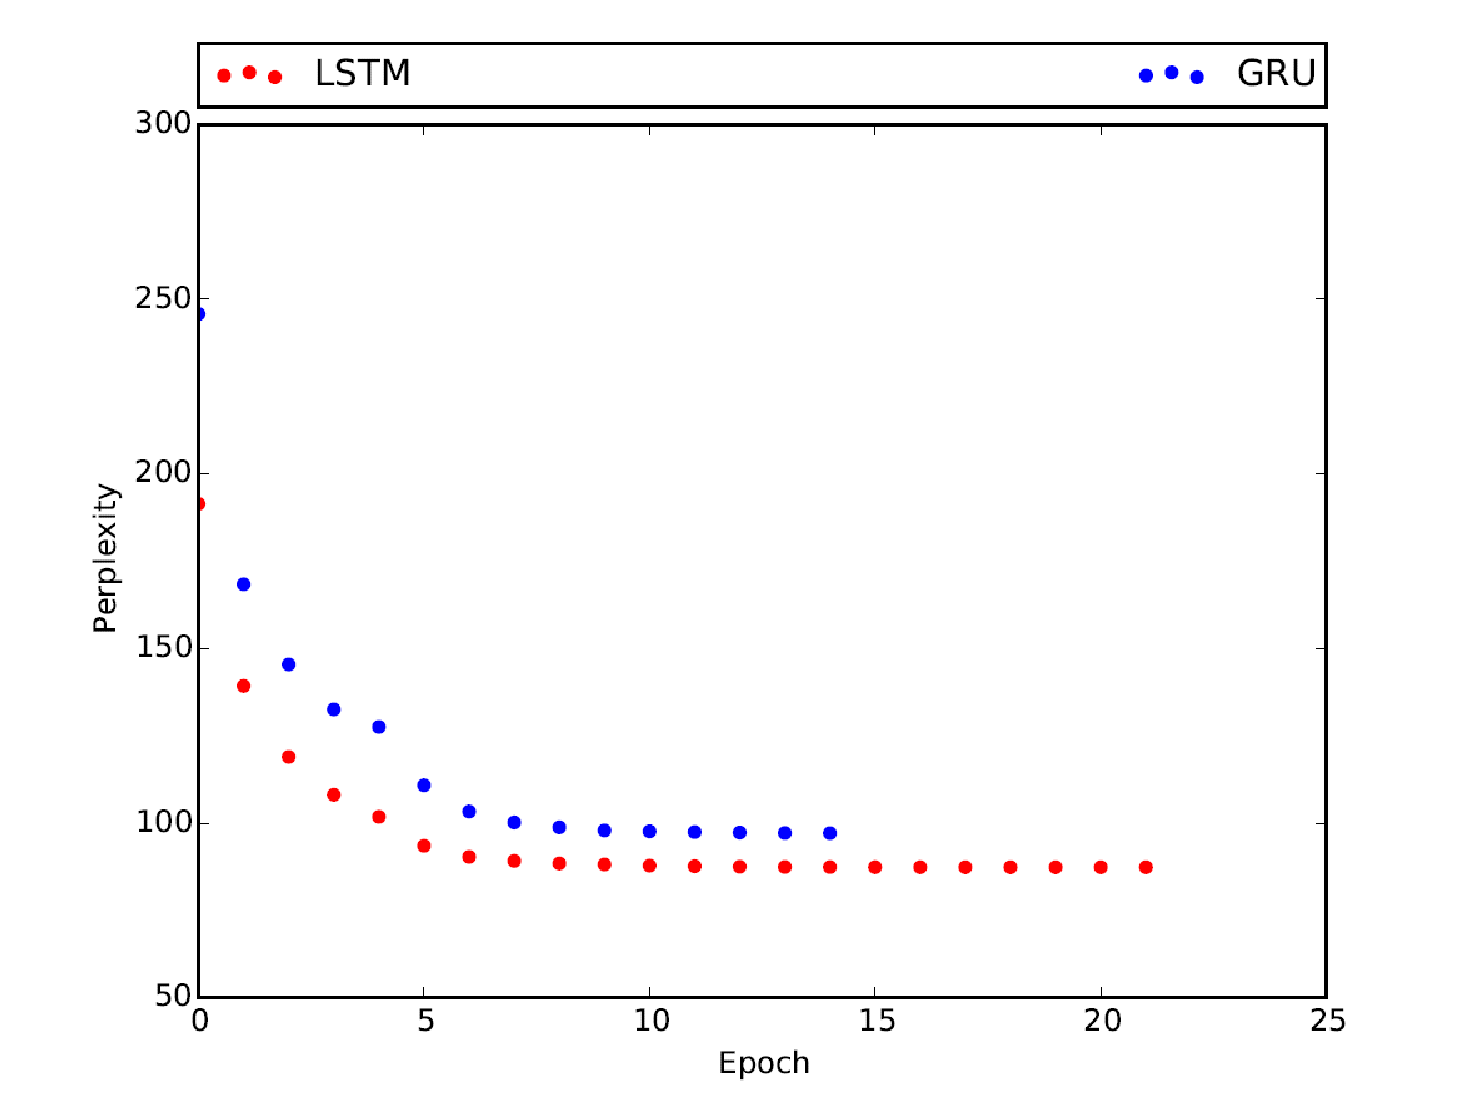
\includegraphics[width=0.65\textwidth]{lstmvsgru}
  \caption{LSTM vs GRU sample comparison plot.\label{fig:gru_cell}}
\end{figure}

\end{document}
